% T4 family (a): a GRAPHICAL-MODEL framework figure, drawn with the bayesnet
% TikZ library (from tikz-bayesnet, distilled in framework-figures.md from
% xinychen/awesome-latex-drawing). Use this shape when the contribution is a
% generative / hierarchical-Bayesian structure, not a pipeline — the "real method
% object" IS the plate structure (latent vs observed variables, repetition).
%
% Build:  pdflatex graphical_model_hero.tex   ->  graphical_model_hero.pdf
% Paper:  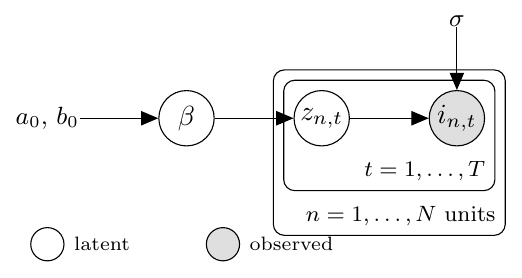
\includegraphics[width=.7\linewidth]{graphical_model_hero.pdf}
%
% Worked example: a hierarchical degradation model — a global wear rate beta is
% drawn from a prior, each unit n has a latent health trajectory z, and the
% sensor current i is the noisy observation (plated over time t, then units n).
\documentclass[border=2mm]{standalone}
\usepackage{tikz}
\usepackage{amsmath, amssymb}
\usetikzlibrary{positioning, calc, bayesnet}
\begin{document}
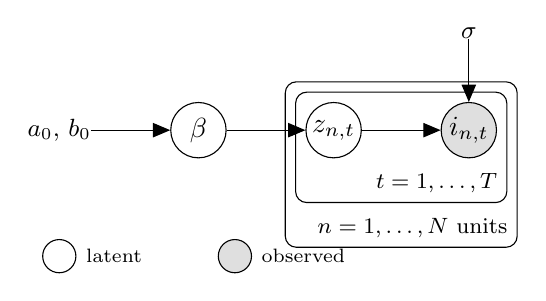
\begin{tikzpicture}[
  node distance = 12mm and 16mm,
  every node/.append style={font=\small},
]
  % --- constants (hyperparameters) and latent / observed variables -----------
  \node[const]                       (hyp) {$a_0,\,b_0$};
  \node[latent, right=of hyp]        (beta){$\beta$};
  \node[latent, right=of beta]       (z)   {$z_{n,t}$};
  \node[obs,    right=of z]          (x)   {$i_{n,t}$};
  \node[const,  above=8mm of x]      (sig) {$\sigma$};

  % --- dependencies ----------------------------------------------------------
  \edge {hyp} {beta};      % prior -> global wear rate
  \edge {beta}{z};         % wear rate -> latent health trajectory
  \edge {z}   {x};         % latent state -> observed current
  \edge {sig} {x};         % observation noise -> observed current

  % --- plates: inner over time t, outer over units n -------------------------
  \plate {pt} {(z)(x)} {\footnotesize $t=1,\dots,T$};
  \plate {pn} {(z)(x)(pt)} {\footnotesize $n=1,\dots,N$ units};

  % --- legend: what filled vs open means (graphical-model literacy) ----------
  \node[latent, scale=0.6, label=right:{\scriptsize latent}] at ($(hyp)+(0,-16mm)$) (ll) {};
  \node[obs, scale=0.6, right=18mm of ll, label=right:{\scriptsize observed}] (lo) {};
\end{tikzpicture}
\end{document}
